\chapter{项目原理}
\label{chap:SomeStuff}

\pagenumbering{arabic}

\section{面向Android终端的隧道原理}

IPv6网络中的用户在希望访问IPv4服务时,将IPv4包封装在IPv6包中发送给一台能够直接访问IPv4服务的服务器。
该服务器将进行实际IPv4资源的访问,然后再将得到的IPv4响应封装在IPv6包中发送回用户。
为了能够通过IPv4地址将IPv4响应返回给相应的用户,IPv4 over IPv6服务器需要维护一个IPv4和IPv6地址的映射表并为需要IPv4 over IPv6服务的用户分配IPv4地址。
本次项目中的IPV4 over IPV6隧道原理如下图所示:
\begin{figure}[!ht]
	\begin{center}
	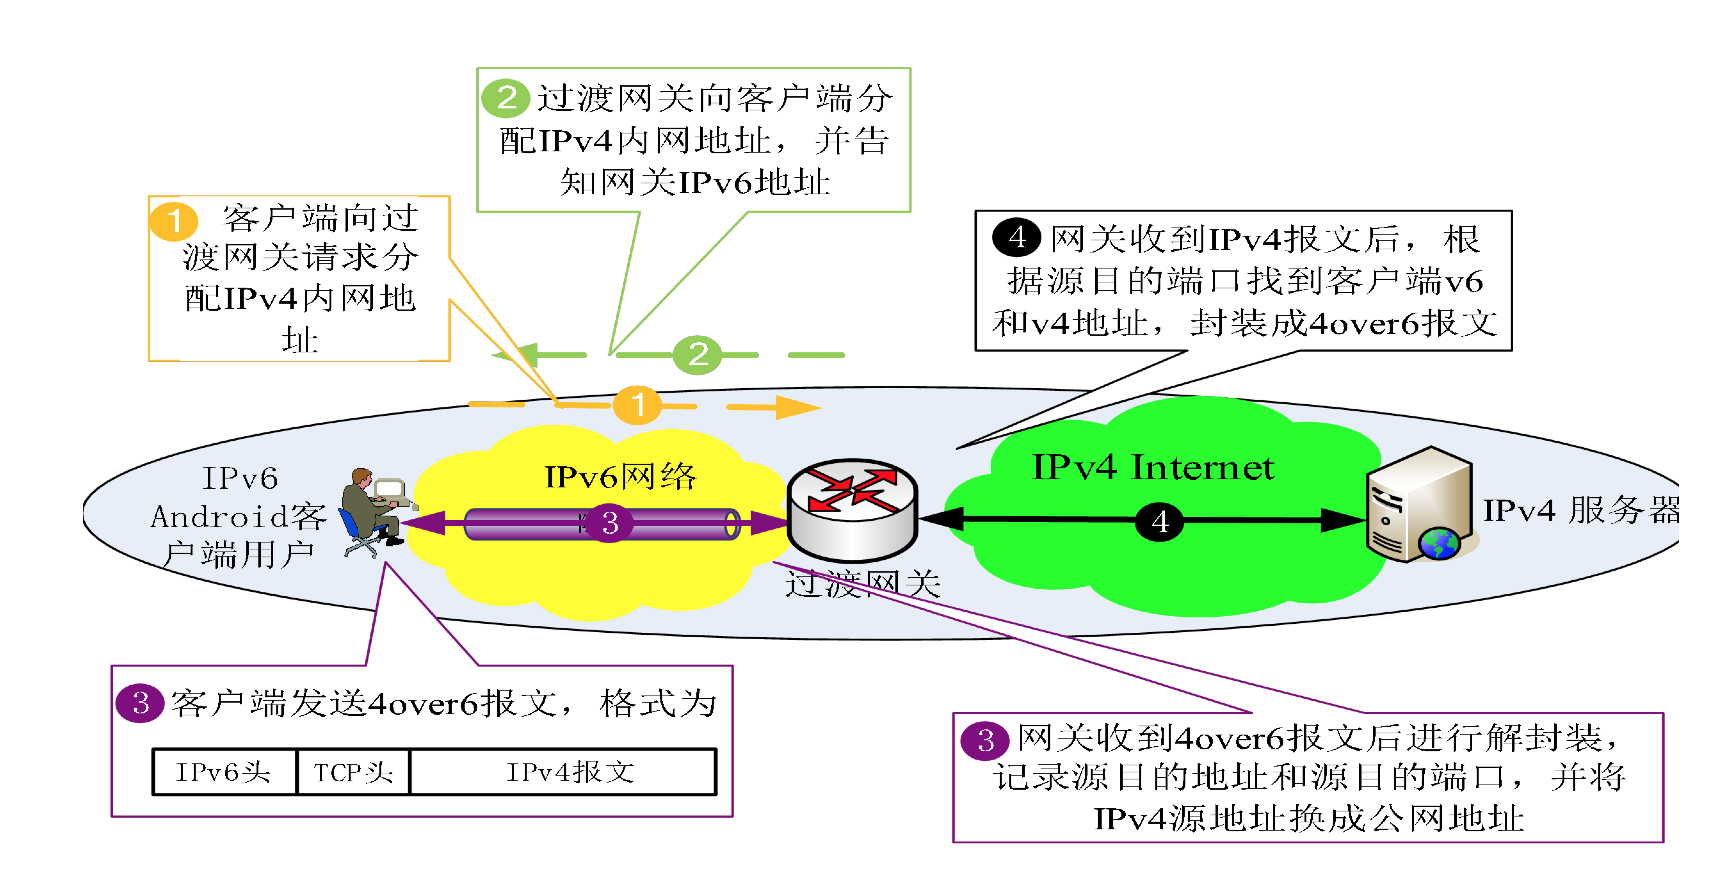
\includegraphics[scale=.58]{4over6.png}
	\end{center}
	\caption{面向Android终端的隧道原理}
	\label{figure:4over6}
\end{figure}
\\ 在本次项目中,我们用到的隧道原理主要是面向Android终端的隧道原理,在面向Android终端的隧道原理中,大致流程为:
安卓客户端首先向过渡网关请求分配 IPv4 内网地址;过渡网关向客户端分配 IPv4 内网地址,并提供对应的 IPv6 网络地址;
接着,安卓客户端发送 IPv4 over IPv6 报文;网关收到报文后解封装,记录源目的地址和源目的端口,并将 IPv4 源地址换成公网地址。
当过渡网关收到来自 IPv4 服务器的报文之后,会根据之前 记录的映射关系,重新封装成 IPv4 over IPv6 报文,发送给对应的内网用户,这样就完成了数据的的转发和接收,用户便可以成 功接收到 IPv4 数据,从而实现通过IPv6网络访问IPv4的功能。


\section{项目网络拓扑}

本次项目中用到的网络拓扑如下图所示:
\begin{figure}[!ht]
\begin{center}
	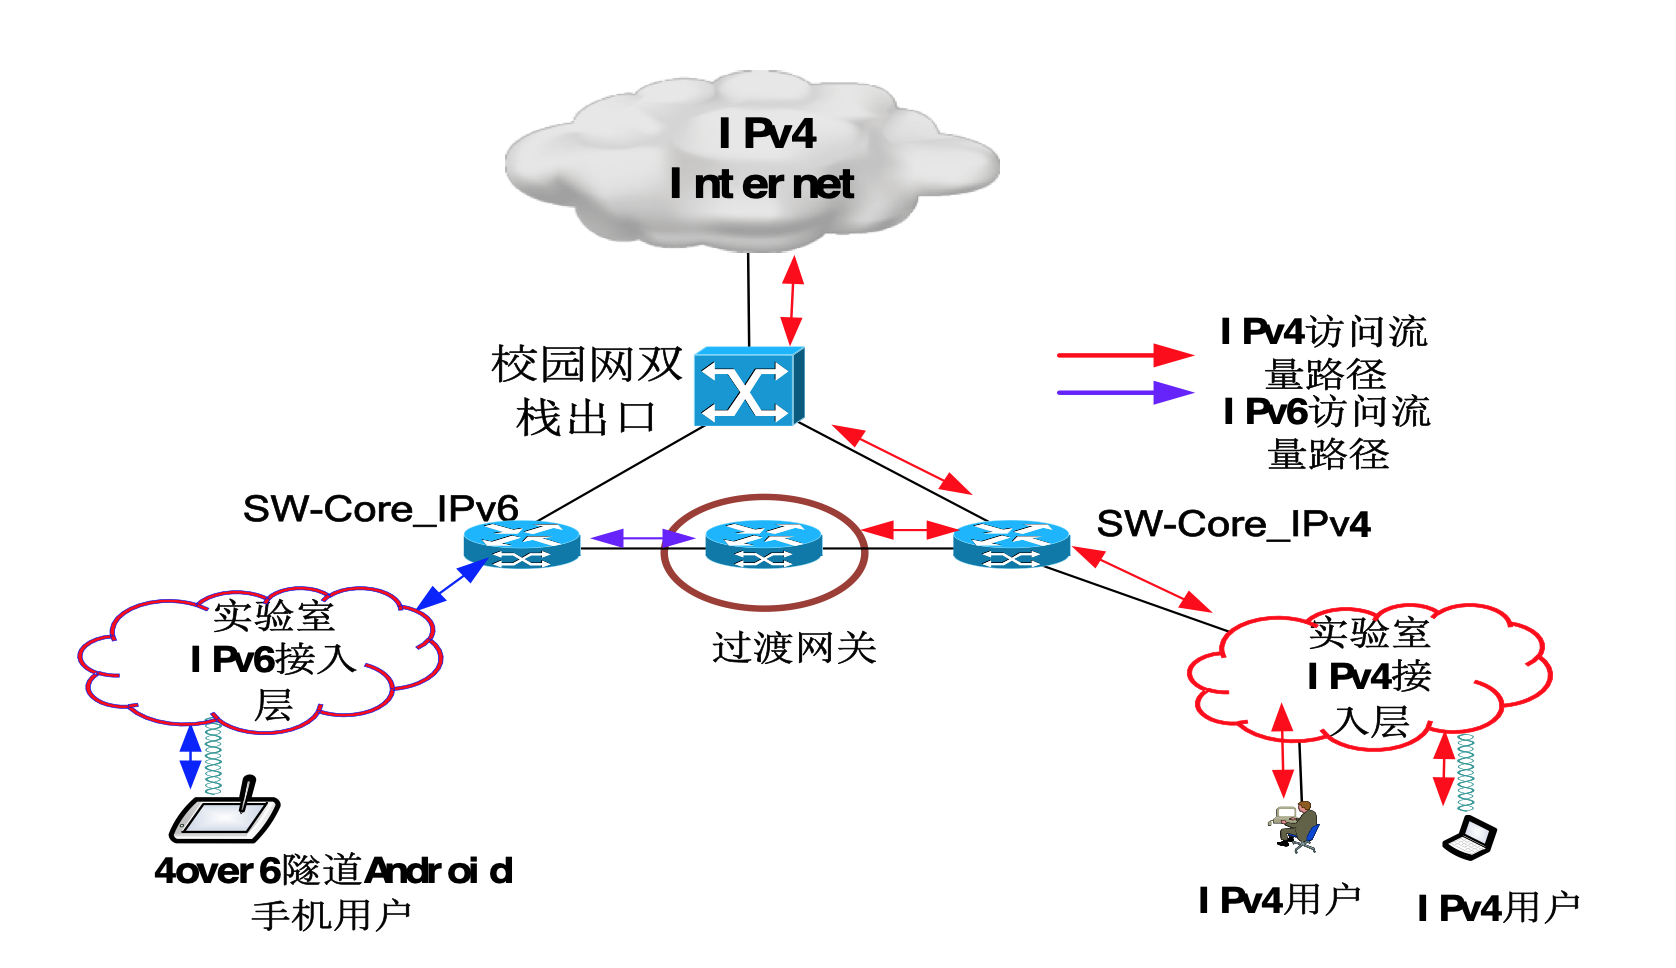
\includegraphics[scale=.58]{network.png}
    \end{center}
    \caption{项目网络拓扑图}
    \label{figure:network}
\end{figure}

\section{安卓VPN Service原理}

VPN Service是一个android自带的vpn服务类,它可以在你不root手机的情况下,实现对你手机流量控制。可以通过设置对指定应用流量的拦截,也可以做全局操作。
如果你的应用是想要拦截网络,或者想要,获取网络数据,转发网络数据,就可以通过这个去做。VPN Service 会监控所有的网络进程,并可以进行 IP 隧道处理。
当我们发送数据时,可以使用 IPv6 包装要发送的报文并发送给网关。
当我们接收数据时,可 以将 IPv4 的报文从数据包中剥离出来。
本次项目中,安卓客户端需要完成 IPv4 over IPv6 报文的封装和解封装,我们采用了 VPN Service 来进行实现。
VPN Service 是安卓的一套 API 接口,方便编程人员创 建 VPN 服务。
打开服务之后,安卓系统将所有的应用程序发送的 IP 包都根据 iptables 使用 NAT 转发到 TUN,其端口为 tun0。
当打开 VPN Service 之后,我们可 以获取 tun0 的文件描述符,这样就可以读取或写入数据以实现发送或者接收数据。

Android设备上,已经使用了VpnService框架,建立起了一条从设备到远端的VPN链接
\begin{itemize}
\item 应用程序使用socket,将相应的数据包发送到真实的网络设备上
\item Android系统通过iptables,使用NAT,将所有的数据包转发到TUN虚拟网络设备上去,端口是tun0
\item VPN程序通过打开/dev/tun设备,并读取该设备上的数据,可以获得所有转发到TUN虚拟网络设备上的IP包
\item VPN数据可以做一些处理,然后将处理过后的数据包,通过真实的网络设备发送出去
\end{itemize}

\section{NDK 和 JNI}
在本次项目中,由于经常要和以字节为单位的数据打交道,并且需要精细地管理 内存,因此我们采用 C 来实现 IPv4 over IPv6 的核心功能。
要在以 Java 为语言的安卓 环境中使用 C 来进行编程,因此我们需要使用 JNI 和 NDK。

NDK 是Native Develop Kit的含义,从含义很容易理解,本地开发。大家都知道,Android 开发语言是Java,不过我们也知道,Android是基于Linux的,其核心库很多都是C/C++的,比如Webkit等。那么NDK的作用,就是Google为了提供给开发者一个在Java中调用C/C++代码的一个工作。NDK本身其实就是一个交叉工作链,包含了Android上的一些库文件,然后,NDK为了方便使用,提供了一些脚本,使得更容易的编译C/C++代码。总之,在Android的SDK之外,有一个工具就是NDK,用于进行C/C++的开发。一般情况,是用NDK工具把C/C++编译为.co文件,然后在Java中调用。

JNI,全称为Java Native Interface,即Java本地接口,JNI是Java调用Native 语言的一种特性。通过JNI可以使得Java与C/C++机型交互。即可以在Java代码中调用C/C++等语言的代码或者在C/C++代码中调用Java代码。由于JNI是JVM规范的一部分,因此可以将我们写的JNI的程序在任何实现了JNI规范的Java虚拟机中运行。同时,这个特性使我们可以复用以前用C/C++写的大量代码JNI是一种在Java虚拟机机制下的执行代码的标准机制。代码被编写成汇编程序或者C/C++程序,并组装为动态库。也就允许非静态绑定用法。这提供了一个在Java平台上调用C/C++的一种途径,反之亦然。
